\documentclass[a4paper,10pt]{article}
\usepackage[utf8]{inputenc}

\usepackage{polyglossia}
\setotherlanguage{english}
\setdefaultlanguage{russian}

\usepackage{adjustbox}
\usepackage{graphicx}

\usepackage{fontspec}
\usepackage{xunicode}
\usepackage{xltxtra}
\usepackage{libertine} 
\usepackage{indentfirst}
\usepackage{amsmath}
\usepackage{amsfonts}
\usepackage{enumitem}


%opening
\title{ДЗ 3}
\author{Михаил Воронов}

\begin{document}

\maketitle

\section{}
$$ f(x, y) = \sqrt{xy} $$

Первое, что можно сразу заметить, это то, что у линий уровня удет иметь место симметрия по $ y = -x$.

$$ y = \frac{f^2(x, y)}{x} $$

Итак, мы знаем, что линии уровня будут гиперболой с коэффициентом равным выбранной константе в квадрате.

Возьмём значения $0$, $1$ и $2$: $(0, 0)$, $y = \frac{1}{x}$, 
$y = \frac{4}{x}$. Построим график:

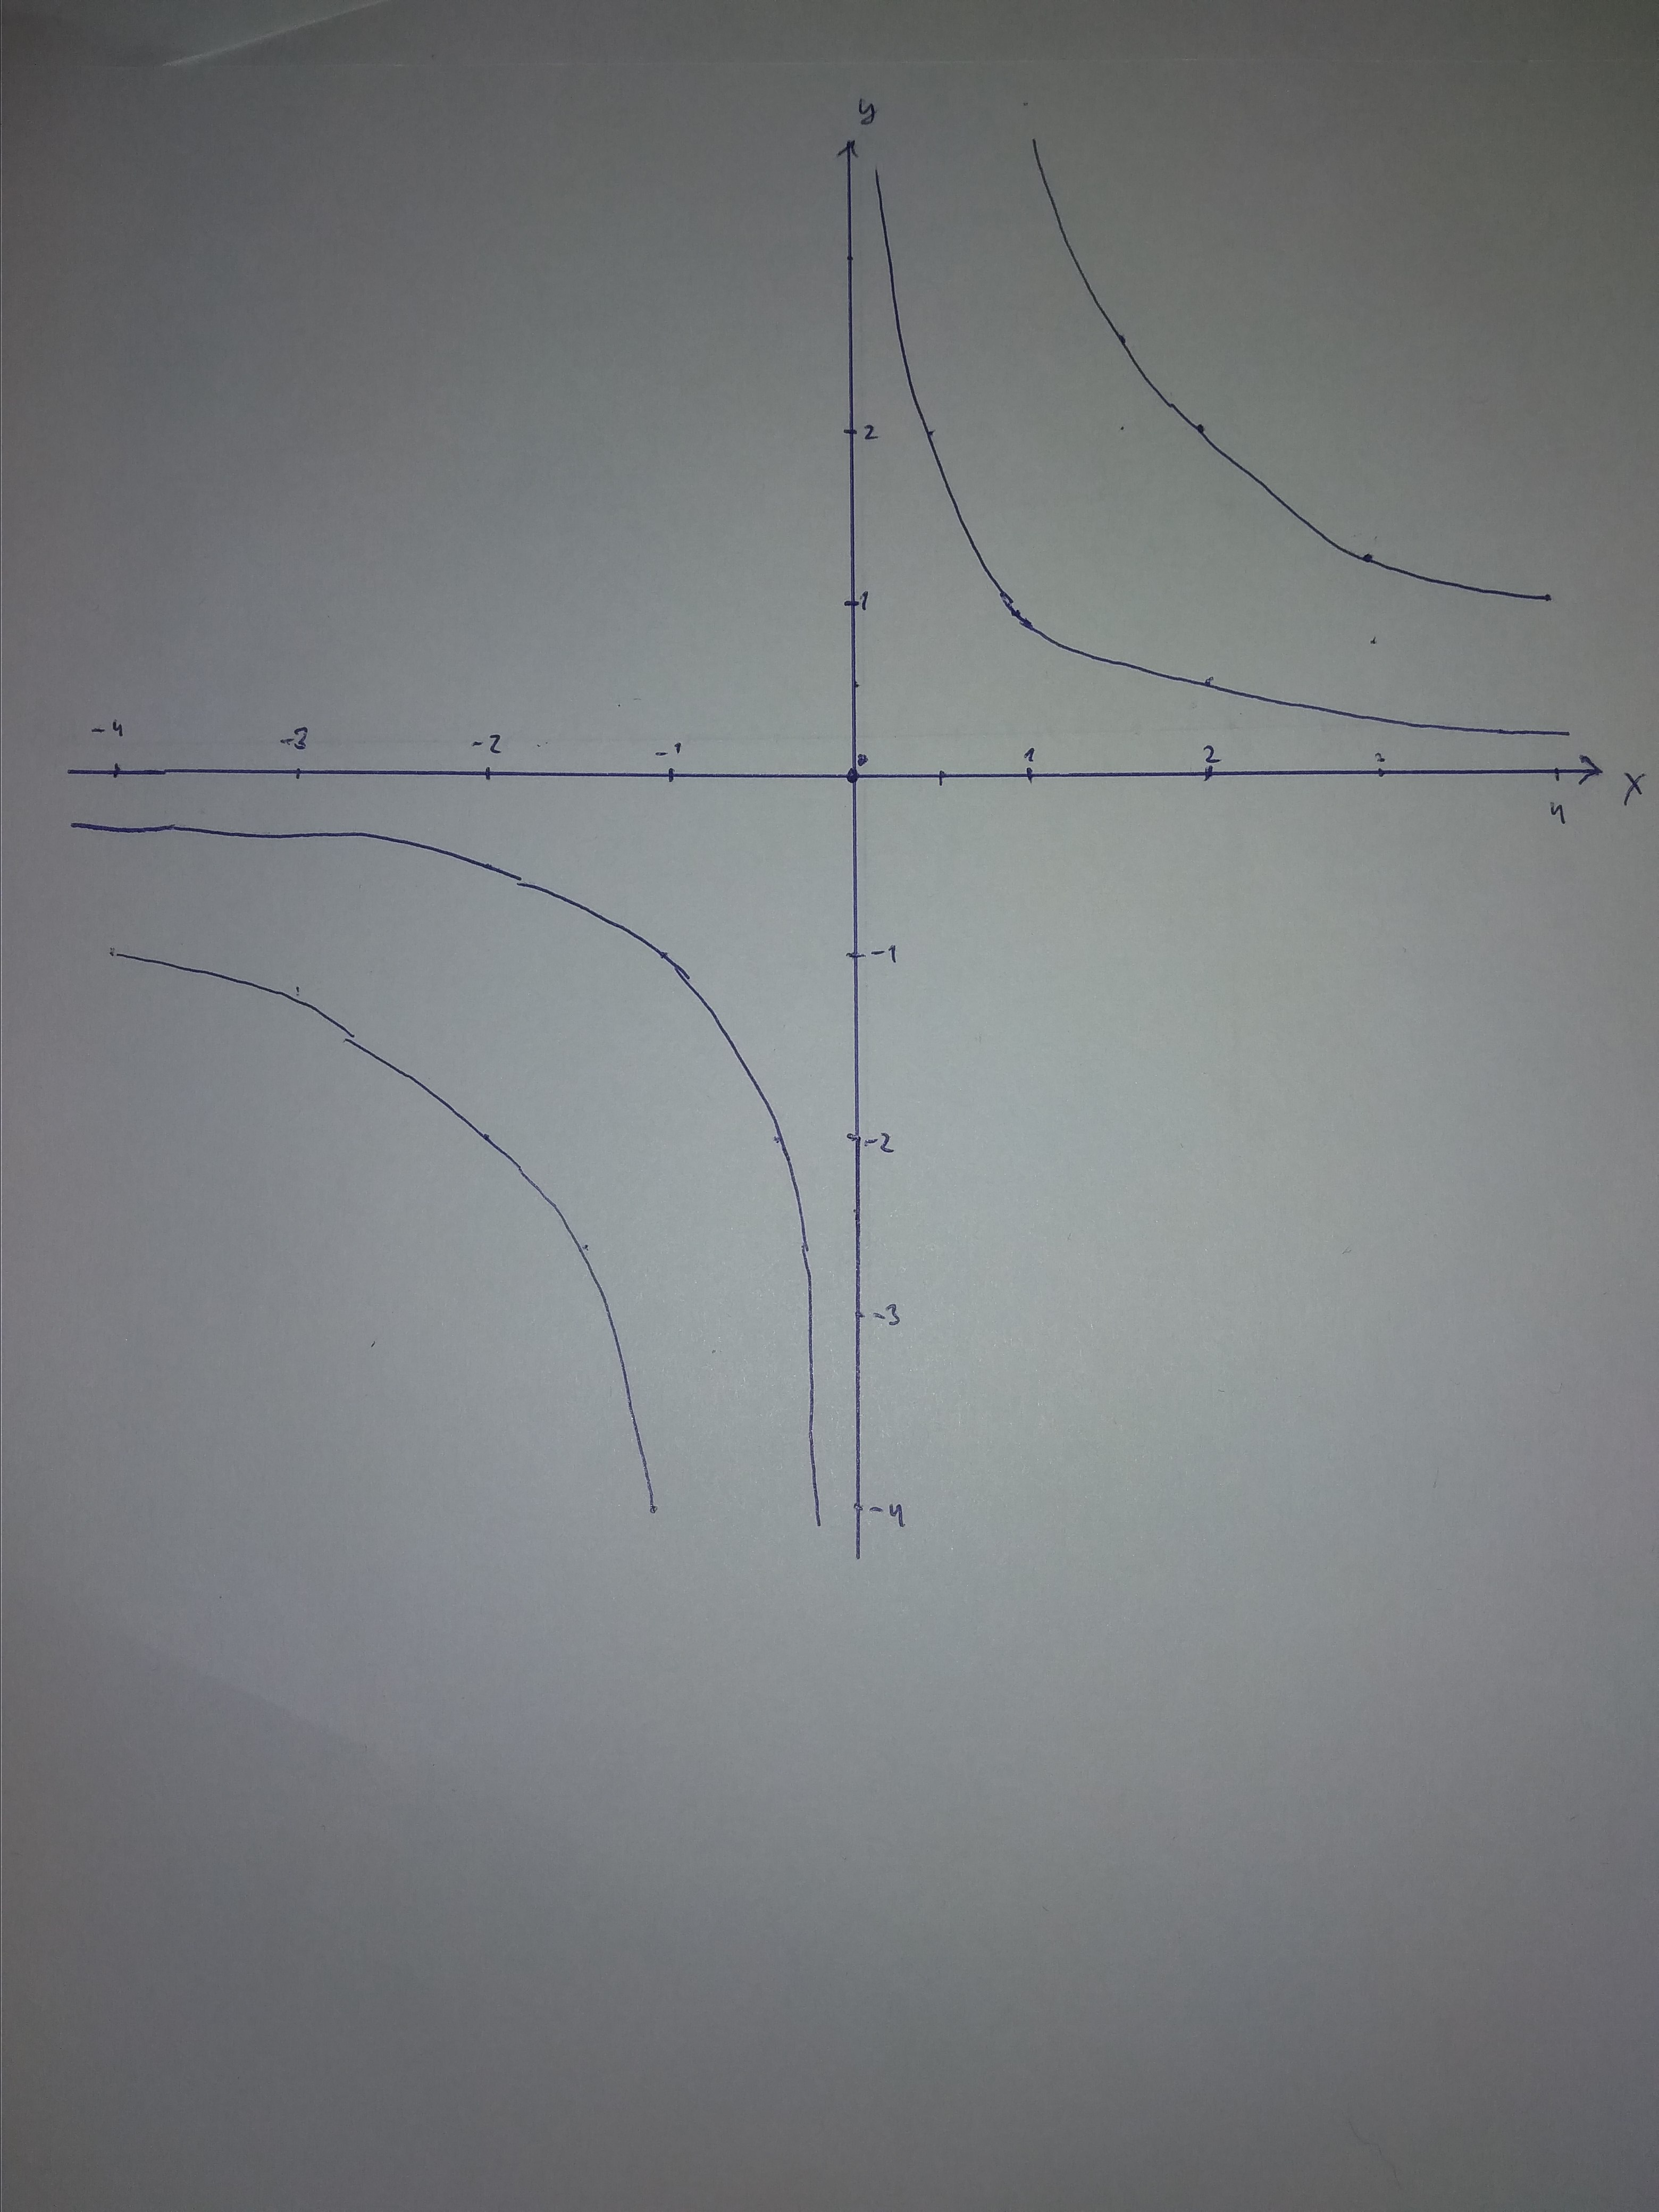
\includegraphics[width=\textwidth]{gr.jpg}

\section{}

$$ f(x, y) = x^2 − xy + y^2 $$

Найдём частные производные:
$$ f^{'}_x(x, y) = 2 - y \big|_{(-1, 2)} = 0 $$
$$ f^{'}_y(x, y) = -x + 2y \big|_{(-1, 2)} = 5 $$

Вспомним формулу производной в точке по направлению вектора:
$$
f^{'}_v = f^{'}_x(x, y)\big|_{A} 
cos\bigg(\frac{v_x}{|v|}\bigg)
+ f^{'}_y(x, y)\big|_{A}
cos\bigg(\frac{v_y}{|v|}\bigg)
$$

Заметим, что первое слагаемое в любом случае будет равно нулю. Значит, производная будет максимальной тогда, когда второе слагаемое будет максимальным. Итак, нам нужен единичный вектор, у которого будет максимальное значение $y$: это вектор $(0, 1)$.

Ответ: $(0, 1)$.

\section{}

Найдём частные производные:
$$ f^{'}_x(x, y) = 4x - 12y + 4 $$
$$ f^{'}_y(x, y) = 3y^2 - 12x - 12 $$

Найдём критические точки:
\begin{equation*}
 \begin{cases}
  4x - 12y + 4 = 0
  \\
  3y^2 - 12x - 12 = 0
 \end{cases}
\end{equation*}
$$ x = 3y - 1 $$
$$ y^2 - 12y = 0 $$
$$ y(y - 12) = 0 $$
\begin{equation*}
 \begin{cases}
  x = -1, y = 0
  \\
  x = 35, y = 12
 \end{cases}
\end{equation*}

Итак, две критические точки: $(-1, 0, 6)$ и $(35, 12, -858)$.

Найдём частные производные второго порядка:
$$ f^{''}_{xx} = 4 $$
$$ f^{''}_{xy} = -12 $$
$$ f^{''}_{yy} = 6y $$

Теперь можно проверять точки.

Начнём с первой. Правда ли, что:
$$
f^{''}_{xx}\big|_{(-1, 0)}
f^{''}_{yy}\big|_{(-1, 0)}
- \big(f^{''}_{xy}\big|_{(-1, 0)}\big)^2
> 0
\equiv
-(-12)^2 > 0
\equiv
-144 > 0
$$

Не правда. Значит, это седловая точка, а не экстремум.

Вторая точка. Правда ли что:
$$
f^{''}_{xx}\big|_{(35, 12)}
f^{''}_{yy}\big|_{(35, 12)}
- \big(f^{''}_{xy}\big|_{(35, 12)}\big)^2
> 0
\equiv
- 12 \times 6 \times 4 - 144 > 0
\equiv
144 < 288
$$

Правда. $ f^{''}_{xx}\big|_{(35, 12)} = 4 > 0 $, значит, это минимум.

Ответ: имеется минимум в точке $(35, 12, -858)$ и седловая точка $(-1, 0, 6)$.

\section{}

$$ f(x, y) = ye^{xy} $$
$$ x_0 = 0 $$
$$ y_0 = 1 $$
$$ z_0 = 1 $$

Вспомним уравнение касательной плоскости в общем виде:
$$ z - z_0 = f^{'}_x(x_0, y_0, z_0)(x - x_0)
+ f^{'}_y(x_0, y_0, z_0)(y - y_0) $$

Найдём частные производные:
$$ f^{'}_x(x, y) = ye^{xy}y = y^2e^{xy} $$
$$ f^{'}_y(x, y) = e^{xy} + e^{xy}xy $$

Остаётся подставить в формулу:
$$ z - 1 = 1^2e^{0}(x) + (e^{0} + e^{0}0)(y - 1) $$
$$ z - 1 = x + y - 1 $$
$$ z = x + y $$

Ответ на пункт \textit{a}: $x + y$.

У нас теперь есть касательная плоскость в точке $(0, 1)$, а нам требуется найти линейное приближение для точки $(-0.1, 1.1)$: достаточно близко для того, чтобы сделть вид, что это точка лежит на найденной плоскости.
$$ f(-0.1, 1.1) \approx x_0 + y_0 = -0.1 + 1.1 = 1 $$

Ответ на пункт \textit{b}: $ f(-0.1, 1.1) \approx 1 $.

\end{document}
